% !TEX root=../main.tex



\section{Example}
\label{sec:example}

In this section we develop an example program to demonstrate the capabilities of \TOPHAT.
The example is a small flight booking system.
It demonstrates communication on all three levels: with the environment, across control flow, and alongside it.
Also, it shows synchronisation and input validation.

The requirements of the application are as follows.
\begin{enumerate*}
  \item A user has to enter a list of passengers for which to book tickets.
  \item At least one of these passengers has to be an adult.
  \item After a valid list of passengers has been entered, the user has to pick seats.
  \item Only free seats may be picked.
  \item Every passenger must have exactly one seat.
  \item Multiple users should be able to book tickets at the same time.
\end{enumerate*}

For this example we assume that the host language has lists and four functions on them: \TS{all}, \TS{any}, \TS{intersect}, and \TS{difference}.
The functions \TS{all} and \TS{any} check if all or any elements in a list satisfy a given predicate.
The functions \TS{intersect} and \TS{difference} compute the set-intersection and set-difference of two lists.
%%NOTE: After Peter's comments symbols are not clear --TS
We also make use of string equality ($\equiv$), dereferencing ($!$), reference assignment ($:=$), and expression sequencing ($;$).
For brevity, we omit the type annotations of variable bindings.


\begin{figure}[b]
  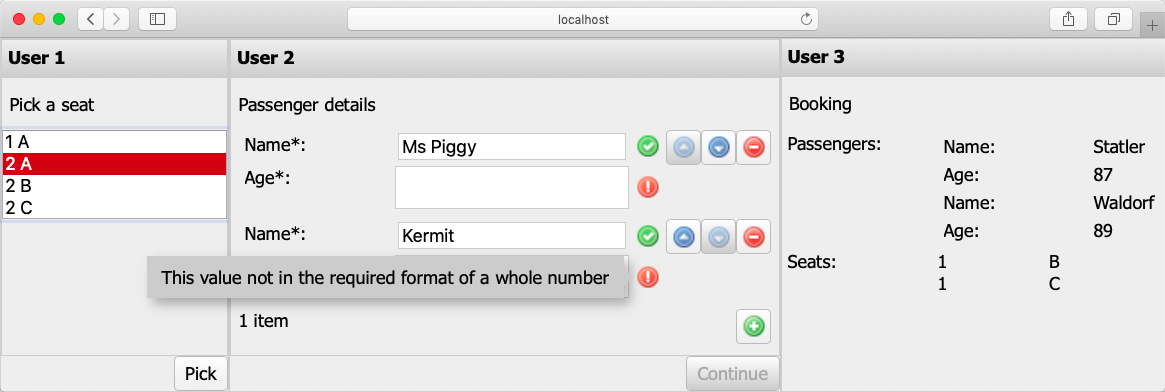
\includegraphics[width=0.8\columnwidth]{figures/flight-booking.png}
  \caption{
    Running web application of the flight booking example using a translation to \ITASKS.
    It shows three users booking a flight simultaneously.
    The first user entered name and age and continued picking seats.
    The second is entering details of two passengers.
    The ages are not filled in, therefore the \TS{Continue} button is disabled.
    The message bubble shows that the \TS{age} field only accepts integer values.
    The third user finished a booking,
    therefore, the first user can not pick seats \smallcaps{1b} and \smallcaps{1c} any more.
  }
  \label{fig:flight-booking}
\end{figure}


\begin{example}[Flight booking]
\label{exm:flight-booking}

We start by defining some type aliases.
A passenger is a pair with name and age.
A seat is a pair with a row number and a seat letter.
\begin{TASK}
  type Passenger = String * Int
  type Seat = Int * String
\end{TASK}

Choosing seats requires reading and updating shared information.
The list of free seats is stored in a reference. % called \TS{freeSeats}.
\begin{TASK}
  let freeSeats = ref [<<1,"A">>, <<1,"B">>, <<1,"C">>, ...]
\end{TASK}

Now we develop our workflow in a top-down manner.
Our flight booking starts with an interactive task \TS{enter (List Passenger)}, where users can enter a list of passengers.
A task $\Enter \tau$ is an empty editor that asks for a value of the given type $\tau$.
Passengers are valid if their name is not empty and their age is at least 0.
Lists of passengers are valid if each passenger is valid, and at least one of the passengers is an adult.
When the user has entered a valid list of passengers, the step after \TS{>>?} becomes enabled,
and the user can proceed to picking seats.
\begin{TASK}
  let valid = \p. not (fst p == "") /\ snd p >= 0 in
  let adult = \p. snd p >= 18 in
  let allValid = \ps. all valid ps /\ any adult ps in
  let bookFlight = enter (List Passenger) >>? \ps.
    if allValid ps then chooseSeats ps else fail
\end{TASK}
A selection of seats is correct if every entered seat is free.
\begin{TASK}
  let correct = \ss. intersect ss !freeSeats == ss in
  let chooseSeats = \ps. enter (List Seat) >>? \ss.
    if correct ss /\ length ps == length ss then confirmBooking ps ss else fail
\end{TASK}

The function \TS{confirmBooking} removes the selected seats from the shared list of free seats,
and displays the end result using an editor, denoted by \TS{edit}.
\begin{TASK}
  let confirmBooking = \ps. \ss.
    freeSeats := difference !freeSeats ss; edit <<ps, ss>>
\end{TASK}
% It uses a function \TS{difference}, which removes all elements from the second list from the first list.

The main task starts three \TS{bookFlight} tasks,
which could be performed by three different users in parallel.
\begin{TASK}
  bookFlight <&> bookFlight <&> bookFlight
\end{TASK}
A screenshot of the running application is shown in \cref{fig:flight-booking}.

All instances of the \TS{bookFlight} task have access to the shared list of free seats.
Rewriting the example in a calculus without side effects would not only be cumbersome,
obfuscating the code with explicit threading of state,
but it would be impossible to model the parallel execution of three \TS{bookFlight} tasks.
It is not known upfront which task will finish first,
and thus it is not possible to thread the free seat list between the parallel tasks.

\end{example}
